% !TeX spellcheck = english
% !TEX root = thesis.tex
\section{\hlr{Fabrication of crystalline silicon nanoparticles by femtosecond laser ablation}}
\label{sec:Ablation}
        The first part of the project was to develop a new, simple, method of fabricating crystalline dielectric
    nanoparticles. The idea was to use controlled laser ablation~--- a very simple technique~--- to produce the particles.
    Previous work on the topic\cite{kuznetsov2012magnetic, zywietz2014laser} has shown that it is possible to fabricate single particles
    of a certain size.

        We ended up developing two different methods to fabricate crystalline nanoparticles~--- direct laser writing of crystalline
    nanoparticles out of a thin film of amorphous silicon (adapted from a method used for plasmonic nanoparticles\cite{makarov2016controllable,
    dmitriev2016direct}), and a forward transfer of nanoparticles by single femtosecond laser pulses
    from a transparent substrate with a a thin film of amorphous silicon to an arbitrary acceptor substrate. The second method is
    similar to the the one presented in \cite{zywietz2014laser}, but doesn't require any additional annealing steps to achieve
    nanoparticle crystallinity and isn't limited to transparent acceptor substrates.

    \begin{figure}[h!]
            \begin{center}
                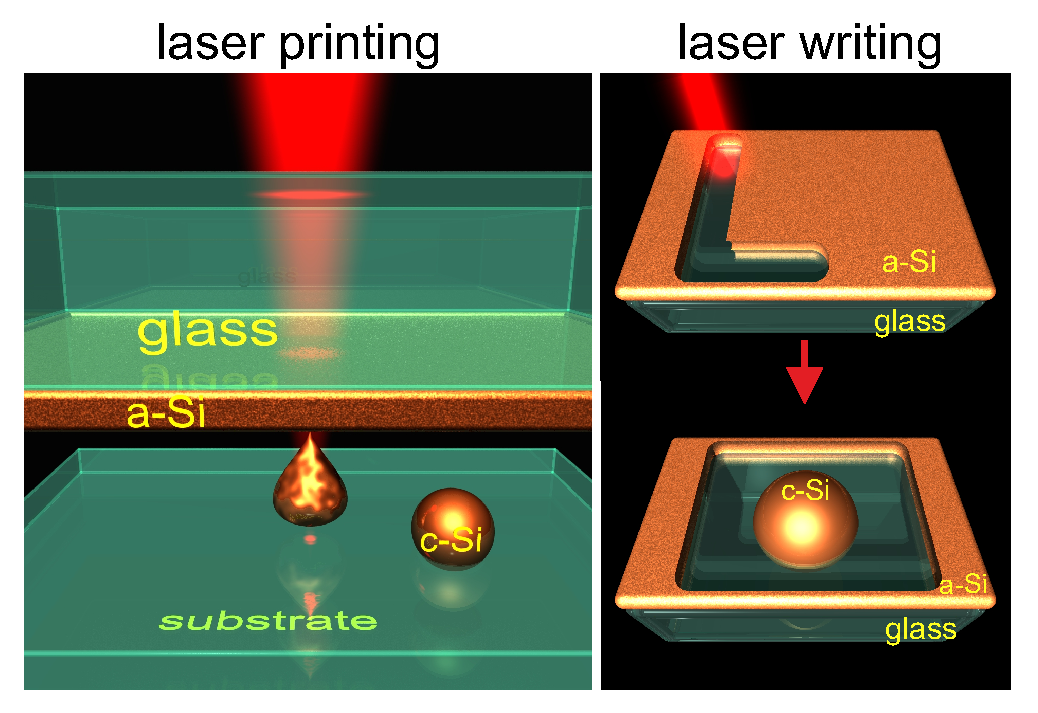
\includegraphics[width=0.5\textwidth]{figs/methods/LaserPrinting.eps}
            \end{center}
            \caption{Geometry of laser-ablation based fabrication methods of crystalline nanoparticles from amorphous
                        thin films.}
            \label{fig:LaserPrinting}
    \end{figure}

    \subsection{\hlb{Generation of femtosecond laser pulses}}
            Femtosecond laser pulse generation is usually done using chirped pulse amplification. A mode-locked seed laser is used
        to generate a train of low-power femtosecond pulses, which are then temporally streched, amplified, compressed and output
        from the laser system. This is necessary, because the final, compressed femtosecond pulse can have extremely high peak power,
        which would damage the amplification system\cite{harilal2014femtosecond}.
            The compression and streching is done by using dispersion to cause different wavelengths of light to travel different distances.
        This is usually accomplished using either two prisms and a mirror or two diffraction gratings and a mirror, though, using engineered
        dispersion in optical fibers is also possible\cite{harilal2014femtosecond}.
            \hlr{Our femtosecond laser system, Femtosecond Oscillator TiF-100F by Avesta Poject, is a Ti:Sapphire laser pumped by a Nd:YLF fequency
        doubled laser, emitting laser pulses at a central wavelength of $800~\si{nm}$, with pulse duration of $100~\si{fs}$, and repetition
        frequency of $80~\si{MHz}$}.

    \subsection{\hlb{Ultrashort-pulse laser ablation}}
            Laser ablation by ultrashort pulses, femto- and picosecond pulses, is a very efficient technique of patterning materials, because
        the short pulse length minimizes the influence of heat conduction on the ablated volume~--- keeping the ablation very localized and
        controlled.

            In metals and semiconductors having a large concentration of conduction band electrons, most of the light from the pulse is
        absorbed by conduction band electrons. The conduction band electrons thermalize within a timeframe of $10$fs-$1$ps, while thermalization
        between the electrons and the lattice is much slowers, on the order of $1-100$ps, meaning that after the absorbtion of the laser pulse,
        we have a non-equilibrium state of a hot electron gas at temperature $T_e$ and a cold lattice at $T$. \cite{bauerle2013laser}

        The evolution of the temperature of the electron gas and the lattice can be described by the following heat equations:

        \begin{align}
            C_e \frac{\partial T_e}{\partial t} &= \nabla (\kappa_e \nabla T_e) - \Gamma_{e-ph}(T_e - T) + Q(x_\alpha, t) \label{ablation:e-heat} \\
            C \frac{\partial T}{\partial t} &= \nabla (\kappa \nabla T) + \Gamma_{e-ph}(T_e - T) \label{ablation:heat}
        \end{align}

        With $C_e, C$ as the heat capacities of the electron gas and the lattice. For a 1D approximation, the source term can
        be written as
        \begin{align}
            Q(z,t) = \alpha A I(t) \exp(-\alpha z)
        \end{align}

        For femtosecond pulses, heat conduction in within the lattice (first right-hand term of Eq.~\ref{ablation:heat}) can be ignored.
        Because the heat capacity of the electron gas is much smaller than that of the lattice, $C_e \ll C$,  the electron gas can
        be heated to very high transient temperatures.

        \begin{align}
           C_e &= C_0 T_e, \quad T_e \ll T_{Fermi} \equiv \frac{E_F}{k_B} \\
           C_0 &= \frac{\pi^2 N_e k_B}{2T_F} \\
           C &= \const, \quad T > \theta_{Debye}
        \end{align}

        The non-equilibrium thermal conductivity of electrons can be approximated by

        \begin{align}
            \kappa_e = \kappa_e(T) \times \frac{T_e}{T}
        \end{align}

        Where $\kappa_e(T)$ is the normal, equilibrium, heat conductivity.

            For femtosecond pulses, the characteristic cooling time of the hot electron gas due to energy exchange with the lattice
        is larger than the pulse duration, $\tau_l \ll \tau_e \equiv \frac{C_e}{\Gamma_{e-ph}}$. For
        $t \ll \tau_e$ or $\Gamma_{e-ph}T_e \ll \frac{C_T_e}{t}$, electron-phonon coupling can be ignored. Another reasonable apporximation,
        considering the thermal diffusivity of electrons $D_e = \frac{\kappa_e}{C_e}$, $D_e\tau_l < \alpha^{-2}$, is to ignore heat
        conduction by electrons. Then Eq.~\ref{ablation:e-heat} simplifies to:

        \begin{align}
            \frac{1}{2}C_0\frac{\partial T_e^2}{\partial t} &= \alpha I_a \exp(-\alpha z) \\
            T_e(t) &= \left(T_0^2 + \frac{2\alpha\phi_a(t)}{C_0}\exp(-\alpha z)\right)^2 \\
            \phi_a(t) &= \int_0^t I_a(t')dt'
        \end{align}

        Where $T_0$ is the initial temperature.

        By the end of the pulse, $t = \tau_l$, we get:

        \begin{align}
            T_e(\tau_l) \approx \left(\frac{2\alpha\phi_a}{C_0}\right)^{\frac{1}{2}}\exp\left(-2\frac{\alpha z}{2}\right)
        \end{align}

        For times $t \geq \tau_l$, Equations \ref{ablation:heat} and \ref{ablation:e-heat}, with $Q = 0$ describe the evolution of the
        two systems. The electron gas then rapidly dumps all the energy to the latice. Continuing to ignore heat conduction, the lattice
        temperature:

        \begin{align}
            T &\approx \frac{\alpha \phi_a}{C}\exp(-\alpha z) \\
            CT &= \int_0^T_e C_e(T_e')dT_e'
        \end{align}

        Significant ablation will occur if $CT \approx \Delta H_v$, where $\Delta H_v$ is the transition enthalpy. All of these approximations
        hold if $T_e \ll \frac{E_F}{k_B}$. The ablated depth is approximately

        \begin{align}
            \Delta h &= \frac{1}{\alpha}\ln\frac{\phi}{\phi_{th}}\\
            \phi_{th} &= \frac{\Delta H_v}{\alpha A}
        \end{align}

        This is a very crude approximation, that disregards energy transport by ballistic and diffusive electron propagation; lattice deformtions,
        thermionic electron emition, etc... A more rigorous treatment would include lattice deformations caused by the heated electron gas. The
        deformation wave caused by the electron gas could cause the metal to fracture and ablate, without significant heating of the lattice itself.

    \subsection{\hlb{Laser transfer of crystalline dielectric particles}}
        % Laser transfer of crystalline nanoparticles was carried out using a
        Single laser pulses were selected by a Pockels cell-based pulse picker (also Avesta Project),
        focused by an oil immersion microscope objective (Olympus $100\times$)
        with a numerical aperture of $\mathit{NA}=1.4$. According to the relation $\emph{d}\approx 1.22\lambda/\mathit{NA}$, the estimated
        diameter of the beam's focal spot size was $d=0.7~\si{\upmu m}$, which was close to the value measured by a method based on
        the dependence of the laser-damaged area on incident laser energy ($0.68~\si{\upmu m}$)~\cite{liu1982simple}.
        The nanoparticles were fabricated from an $80~\si{nm}$ thick a-Si:H film deposited on a fused silica substrate by
        plasma enhanced chemical vapor deposition from a SiH$_{3}$ precursor gas.

            The nanoparticles were fabricated by single laser pulses (from a previously undamaged surface of the a-Si:H film) in a
        forward-transfer geometry, where the receiving substrate is placed under the film with a spacing
        of $\sim 50~\si{\upmu m}$ (figure~\ref{fig:LaserPrinting}(a)). This geometry has an advantage over the back-transfer geometry
        used in \cite{zywietz2014laser}, because of the possibility of transferign nanoparticles onto a wide variety of substrates,
        including opaque and structured samples.

            The silicon nanoparticles were printed at laser energies in the range of $0.5-1.2~\si{nJ}$, providing fluencies in
        the range of $0.12-0.16~\si{J/cm^{2}}$. The fabricated nanoparticles were almost spherical in shape(figure~\ref{fig:Crystallinity}(b))
        and their diameters lie in the range of $50-200~\si{nm}$, depending on the fluence.

    \subsection{\hlb{Laser writing of dielectric particles}}
            The direct laser writing of crystalline Si nanoparticles was carried out from an initially amorphous a-Si:H film.
        The process consists of using a train of femtosecond pulses to cut patches out of the a-Si thin film\cite{makarov2016controllable,
        dmitriev2016direct}. A laser fluence $F\approx100~\si{mJ/cm^{2}}$ provides film heating close to the melting point even in a
        single shot regime, while a pulse train with a $12.5~\si{ns}$ delay between pulses leads to the temperature accumulation
        and exceeding of the ablation threshold. The heat transferring from the ablated area to the surrounding film is accumulated
        much stronger in the cut patches, which are thermally isolated from the rest of the film.
        These micro-patches are unstable at high temperatures and undergo dewetting to a certain number of similar
        nanoparticles~\cite{thompson2012solid}.


\clearpage
